\section{Durchführung}
\label{sec:Durchführung}

\subsection{Fourieranalyse}
\begin{figure}[H]
  \centering
  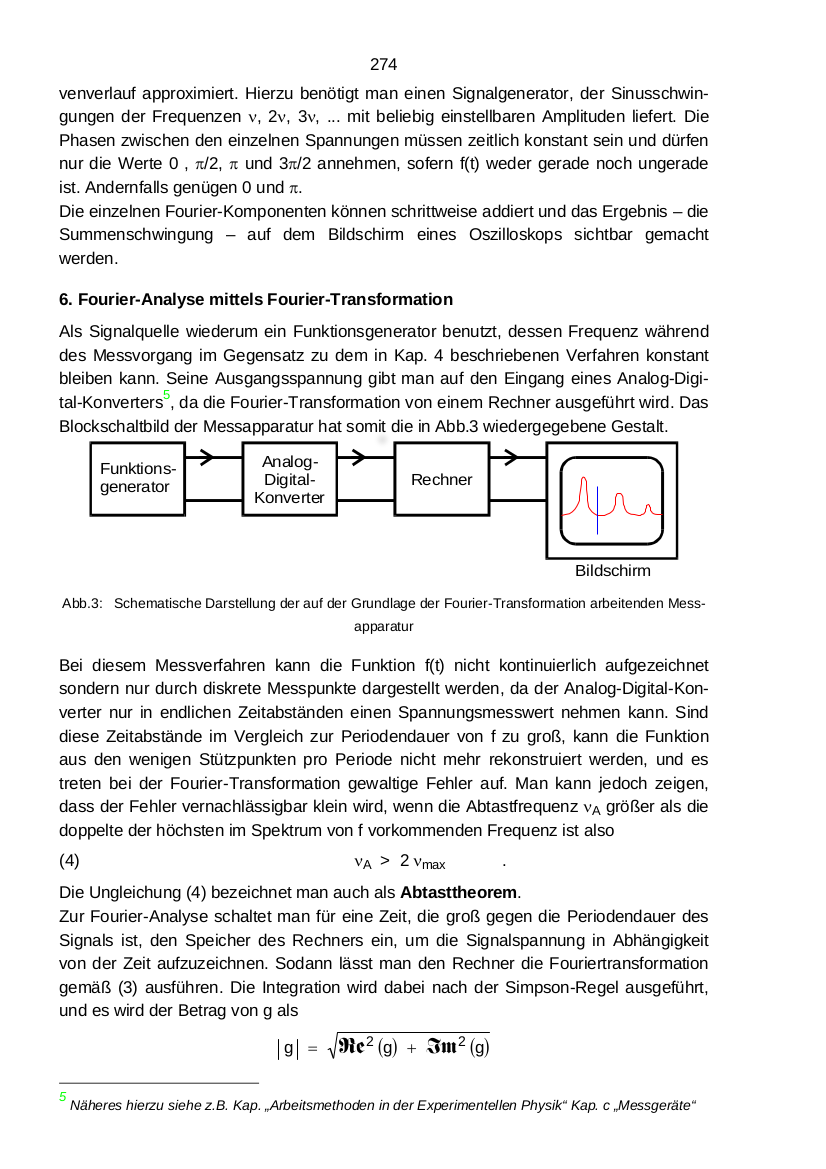
\includegraphics{content/images/analyse2.png}
  \caption{Aufbau zu Fourieranalyse.}
  \label{fig:anal}
\end{figure}
In Abbildung \ref{fig:anal} ist der Versuchsaufbau zur Fourieranalyse
dargestellt. Im Funktionsgenerator werden Rechteck-, Sägezahn- beziehungsweise
Dreiecksspannung generiert und im Analog-Digital-Konverter in ein für einen
Computer erkennbares Signal umgewandelt. Im Rechner findet nun die
eigentliche Fourieranalyse anhand konkreter Messpunkte statt.
Danach wird das Ergebnis als Spektrum auf dem Osziloskop abgebildet
und kann ausgewertet werden, wobei beachtet werden muss, dass die
Spektren nicht konkret sondern als piks angezeigt werden, da der
Computer nur endlich genau Messen kann.

\subsection{Fouriersynthese}
